% !TeX root = cm1005-itp1-notes.tex

\documentclass{article}
\usepackage[utf8]{inputenc}
\usepackage[english]{babel}
\usepackage{xcolor}

\usepackage{minted}
\setminted{fontfamily=tt}
% Disable italics for comments and configure color of code block text
\usepackage{etoolbox}
\BeforeBeginEnvironment{minted}{\def\FancyVerbFormatLine{\def\baselinestretch{1}\small\color{white}}}
\AtBeginEnvironment{minted}{\let\itshape\relax}

\usepackage{graphicx}
\usepackage{tikz}

\usepackage[scaled]{helvet}
\renewcommand*\familydefault{\sfdefault}

\usepackage[hmargin=2.54cm, vmargin=2.54cm]{geometry}

% Define custom color
\definecolor{darkgray}{RGB}{13, 17, 23}
\definecolor{lightgrey}{RGB}{216, 222, 233}

\pagecolor{darkgray}
\color{lightgrey}

\begin{document}

\begin{titlepage}
    \centering
    \vspace*{2cm}
    
    {\LARGE\bfseries CM1005 - Introduction to Programming I}\\[0.8cm]
    {\large\bfseries BSc Computer Science}\\[0.5cm] 
    {\large\textnormal{Nathan Donovan}}\\[1.5cm] 

    
\includegraphics[scale=0.1]{../images/university-of-london-logo.png}\\[1.5cm] 
    {\Large\bfseries University of London}\\[1cm]
    {\large April 2024}

    \vfill
    
\end{titlepage}

\newpage
\section{p5.js - JavaScript Library for Creative Coding}

\subsection*{Using p5.js}
\begin{itemize}
    \item Projects / programs must be opened at the folder level in Brackets.io / other IDE for live preview to work.
    \item Work on sketch.js file only. 
        \begin{itemize}
            \item index.html is boilerplate for the sketch to run as a web page.
            \item p5.min.js is the p5.js library code.
        \end{itemize}
\end{itemize}

\vspace*{0.5cm}
\noindent Function used to set up the sketch, width and height are specified in pixels with the origin (0,0) at the top left hand corner of the browser window:

\vspace*{0.25cm}
\begin{minted}{javascript}
    function setup() {
        createCanvas(width, height);
    }
    \end{minted}


\begin{center}
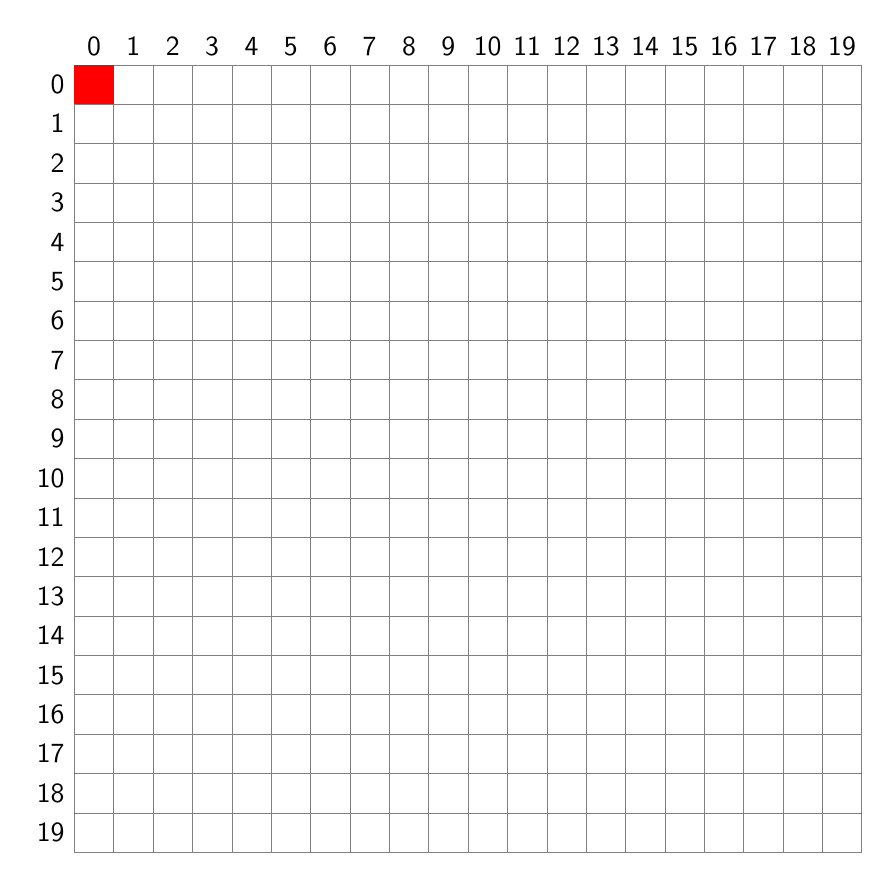
\begin{tikzpicture}[scale=0.50]
    % Draw the 20x20 grid
    \draw[step=1, gray, very thin] (0,0) grid (20,20);
    
    % Highlight the origin (0,0)
    \fill[red] (0,19) rectangle (1,20);

    % Loop for labels on the left axis
    \foreach \y in {0,...,19}
        \node[left] at (0,19.5-\y) {\y};
    
    % Loop for labels on the top axis
    \foreach \x in {0,...,19}
        \node[above] at (\x+0.5,20) {\x};   
\end{tikzpicture}

\vspace*{0.5cm}
Origin pixel highlighted in red at (0, 0), example canvas is 20 x 20 pixels.
\end{center}

\newpage
\subsection*{Drawing and Shape Functions}
\noindent Function used to contain the drawing commands in the sketch:
\begin{minted}{javascript}
    function draw() {
        // Various functions available as part of the p5.js library
    }
    \end{minted}

\noindent Example p5.js shape functions used:

\begin{minted}{javascript}
    // rect() syntax
    rect(x, y, width, height, [tl], [tr], [br], [bl]);
    /*
    tl = top-left radius
    tr = top-right radius
    br = bottom-right radius
    bl = bottom-left radius
    */

    // ellipse() syntax
    ellipse(x, y, width, [height]); // height is optional
    
    // point() syntax
    point(x, y);    // point() is a single pixel unless modified with strokeWeight()
                    // Can only be colored with stroke(), not fill()
    
    // triangle() syntax
    triangle(x1, y1, x2, y2, x3, y3);

    // vertex() syntax
    vertex(x, y);   // Can be used to construct complex shapes
                    // Used exclusively with beginShape() and endShape()
    // Example:
    beginShape();   // fill(), stroke() etc. to be used before beginShape() called
    vertex(x1, y1);  
    vertex(x2, y2);
    vertex(x3, y3);
    endShape();

    // beginShape() syntax
    beginShape([kind]);
    /*
    kind = POINTS, LINES, TRIANGLES, TRIANGLE_FAN, TRIANGLE_STRIP, QUADS, QUAD_STRIP or TESS

    examples shown in p5.js reference documentation
    */

    \end{minted}

\newpage
\subsection*{Colour Functions}
\noindent Example p5.js color functions used:
    
\begin{minted}{javascript}
    // stroke() syntax
    stroke(red, green, blue, [alpha]); // alpha is optional
    // red, green, blue and alpha values are between 0 and 255

    // fill() syntax
    fill(red, green, blue, [alpha]); // alpha is optional
    // red, green, blue and alpha values are between 0 and 255

    // noFill() syntax
    noFill();   // Disables fill color for shapes


\end{minted}



\end{document}
